\section{Results}
\label{sec:results}

%Performance Evaluation, Results, Discussion}

%\textit{owners: Evan: graphs, All: interpretation (2.75 pages)}

\subsection{CX Performance using C and MPI} %%on Single Node}
  \label{sxn:results1}


   
%%  \vspace*{0.1in}

In Table~\ref{tab:single_node}, we show the benefits of the
      optimizations described in
      Sec.~\ref{sxn:single_node_opt}. 
      %%%%
      %%%%
      %%%%
      %to the performance of \textsc{MultiplyGramian} and \textsc{Multiply} on each compute node. 
      %%
      %%
      %The test matrix $\mathcal{A}$ has {\it{m}} = 1.95M, {\it{n}} = 128K,
      %{\it{s}} = 0.004, and {\it{nnz}} = 10$^9$. The parameter
      %{\it{k}} = 32. 
      As far as single-node performance is concerned, we started with a parallelized implementation  
      without any of the described optimizations. %%, and measured the performance (in terms of time taken). 
      We first implemented the multi-core synchronization scheme, wherein a single copy of the
      output matrix is maintained, %% across all the threads (for the matrix multiplication).
      which resulted in a speedup of 6.5X, primarily due to
      the reduction in the amount of data traffic between 
      main memory and caches. 
      %%last-level cache and main memory (there was around 19X measured reduction in traffic). 
      We then implemented our cache blocking scheme, which led to a
      further  2.4X speedup (overall 15.6X).
%%      primarily targeted towards ensuring that the output of the matrix multiplication resides in the caches (since it is
%      accessed and updated frequently). This led to a further 2.4X reduction in run-time, for an overall speedup of around 15.6X.
      We then implemented our SIMD code that sped it up by a further
      2.6X, for an overall speedup of 39.7X. 



%%     Once the memory traffic was optimized for, we implemented our
%%     SIMD code by vectorizing the element-row multiplication-add
%%     operations (described in detail in Sec.~\ref{sxn:single_node_opt}). 
%%     The resultant code sped up by a further 2.6X, for an overall
%%     speedup of 39.7X. Although the effective SIMD width
%% ($\mathcal{S}$ = 4), there are overheads of address computation,
%% stores, and not all computations were vectorized (QR code is still %% scalar).



        As far as the multi-node performance is concerned, 
 on the Amazon EC2 cluster, with 30 nodes (960-cores in total), and
 the 1 TB dataset as input, the C code
 took 151 seconds to perform the CX computation (including the time to load
 the data into main memory). 
 Compared to the Scala code on the same platform (details in the
 next section), we achieved a speedup of 21X.

 Some of these optimizations can be implemented in Spark, such as arranging the
 order of memory accesses to make efficient use of memory. %%of the memory bus.
 However, other optimizations such as sharing the output matrix between threads
 and the use of SIMD intrinsics fall outside the Spark programming model, and would
 require piercing the abstractions provided by Spark and the JVM.
 %to more directly access and manipulate the hardware.
 Thus there is a tradeoff between optimizing performance 
 and the ease of implementation %% and efficient global scheduling, 
 available when expressing programs in the Spark programming model.

 
  \begin{table}
  \begin{center}
  \begin{tabular}{ |c|c| } 
  \hline
  Single Node Optimization & Overall Speedup\\
  \hline
  Original Implementation & 1.0  \\
  Multi-Core Synchronization & 6.5 \\
  Cache Blocking & 15.6 \\
  SIMD & 39.7 \\
  \hline

  \end{tabular}
  \end{center}
  \caption{Single node optimizations to the CX C implementation and
    the subsequent speedup each additional optimization provides.}
  \label{tab:single_node}
  \end{table}
 



  \subsection{CX and PCA Performance Using Spark} %% on Spark} across Multiple Nodes}

  \subsubsection{Spark Phases}
  The CX and PCA algorithms proceed in four distributed phases listed below, along with a small amount of additional local computation.
  \begin{enumerate}
      \item \textbf{Load Matrix Metadata}
         The dimensions of the matrix are read from the distributed filesystem to the driver.
      \item \textbf{Load Matrix}
         A distributed read is performed to load the matrix entries into an in-memory cached
         RDD containing one entry per row of the matrix. PCA uses an additional pass over the matrix to compute and remove the column means.
       \item \textbf{Power Iterations / MultiplyGramian}
         In the case of the CX algorithm, the \textsc{MultiplyGramian} loop (lines 2-5) of
         \textsc{RandomizedSVD} is run to compute an approximate basis $Q$
         of the dominant right singular subspace. For the PCA algorithm, the ARPACK routine calls the \textsc{MultiplyGramian} function
         until the approximate eigenvectors converge to the desired top eigenspace of $AA^T.$
       \item \textbf{Finalization (Post-Processing)}
         In the case of the CX algorithm, right multiplication by $Q$ (line 7) of \textsc{RandomizedSVD} to compute $C$. In the case of the PCA algorithm,
         right multiplication by $V$ followed by some local post-processing to compute the principal components vectors.
  \end{enumerate}

  \subsubsection{Empirical Results}

    \begin{figure} [h!btp]
    \begin{centering}
    \includegraphics[scale=0.4]{images/CX_Strong_Scaling_New_Colors_Axes_Rank_32_Partitions_default.pdf}
    \end{centering}
    \caption{ Strong scaling for the 4 phases of CX on an XC40 for 100GB dataset at $k=32$ and default partitioning as concurrency is increased.} 
    \label{fig:xc40scaling}
    \end{figure} 

Figure~\ref{fig:xc40scaling} shows how the distributed Spark portion of our CX code scales.
We considered 240, 480, and 960 cores.  An additional doubling (to 1920 cores) would be ineffective as there are only 1654 partitions, 
so many cores would remain unused.  
When we go from 240 to 480 cores, we achieve a speedup of 1.6x:
233 seconds versus 146 seconds.  However, as the number of partitions per core drops 
below two, and the amount of computation-per-core relative to communication overhead drops, 
the scaling slows down (as expected).  
This results in a lower speedup of 1.4x (146 seconds versus 102
seconds) from 480 to 960 cores.
We did not produce a similar scaling plot for the PCA experiments, as using less
than the maximum 960 cores results in the dataset (2.2 TB of climate data)
results in the dataset not fitting in memory.

\subsection{CX and PCA Performance across Multiple Platforms}
  \label{sect:h2h}
    
    \begin{figure} [h!btp]
    \begin{centering}
      \includegraphics[scale=0.4]{images/CX_Size_Scaling_EXP_CC_xc40_ec2_Rank_16_and_32_Partitions_default.pdf}
    \end{centering}
    \caption{ Run times for the various stages of computation of CX on the three platforms using $k=16$ and $k=32$ on the 1 TB size dataset, using the default partitioning on each platform.} 
    \label{fig:h2hrank16} 
    \end{figure}

    \begin{figure} [h!btp]
      \begin{centering}
        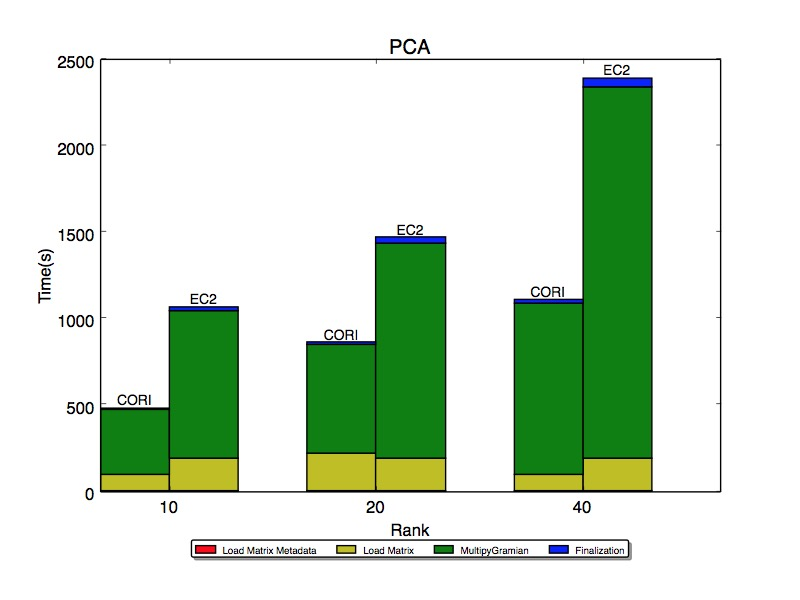
\includegraphics[scale=0.3]{images/phase_stackplot_ec2}
      \end{centering}
      \caption{Run times for the various stages of computation of PCA on the EC2 and Cori platforms using $k=10, k=20,$ and $k=40$ on the 2.2 TB size dataset, using the default partitioning.}
      \label{fig:pca_h2hranks}
    \end{figure}
    
      \begin{table*}
    \begin{center}
    \begin{tabular}{| l | c | c | c | c | c | c |}
    \toprule
    \textbf{Platform} & \textbf{Total} & \textbf{Load} & \textbf{Time Per} & \textbf{Average} & \textbf{Average} & \textbf{Average} \\
                               & \textbf{Runtime} & \textbf{Time} & \textbf{Iteration} & \textbf{Local} & \textbf{Aggregation} & \textbf{Network} \\
                               & & & & \textbf{Task} & \textbf{Task} & \textbf{Wait} \\
    \midrule
    Amazon EC2 \texttt{r3.8xlarge} & 24.0 min & 1.53 min & 2.69 min & 4.4 sec & 27.1 sec & 21.7 sec \\
    \midrule
    Cray XC40 & 23.1 min& 2.32 min & 2.09 min &  3.5 sec & 6.8 sec & 1.1 sec \\
    \midrule
    Experimental Cray cluster & 15.2 min & 0.88 min & 1.54 min &  2.8 sec & 9.9 sec & 2.7 sec \\
   \bottomrule
    \end{tabular}
    \end{center}
    \caption{Total runtime for the 1 TB dataset ($k=16$), broken down into load time and per-iteration time. The per-iteration time is further broken down into the average time for each task of the local stage and each task of the aggregation stage.  We also show the average amount of time spent waiting for a network fetch, to illustrate the impact of the interconnect.}
    \label{tab:h2hres1TB}
    \end{table*}
    
Table~\ref{tab:h2hres1TB} shows the total runtime of CX for the 1 TB dataset on
our three platforms.  The distributed Spark portion of the computation is also
depicted visually in Figure~\ref{fig:h2hrank16} for $k=16$ and $k=32$ on the 1
TB dataset.  All three platforms were able to successfully process the 1 TB
dataset in under 25 minutes.  As the table and figure illustrates, most of the
variation between the platforms occurred during the \texttt{MultiplyGramian}
iterations.  We now explore how the platform differences relate to the performance of the matrix
iterations.

Spark divides each iteration into two stages.  The first \emph{local}
stage computes each row's contribution, sums the local results (the
rows computed by the same worker node), and records these %%locally-aggregated 
results.  The second \emph{aggregation} stage combines all of the workers' locally-aggregated results using a tree-structured reduction.  Most of the variation between platforms occurs during the aggregation phase, where data from remote worker nodes is fetched and combined.  In Spark, all inter-node data exchange occurs via \emph{shuffle operations}.  In a shuffle, workers with data to send write the data to their local scratch space.  Once all data has been written, workers with data to retrieve from remote nodes request that data from the sender's block manager, which in turns retrieves it from the senders local scratch space, and sends it over the interconnect to the receiving node.

Examining our three platforms (Table~\ref{tab:hwspecs}), we notice two key hardware differences that impact shuffle operations:
\begin{itemize}
\item First, both the EC2 nodes and the experimental Cray cluster nodes have fast SSD storage local to the compute nodes that they can use to store Spark's shuffle data.  
  The Cray{\textsuperscript{\tiny\textregistered}}~XC40{\textsuperscript{\tiny\texttrademark}} system's~\cite{alverson2012cray,craycascadesc12} nodes, on the other hand, have no local persistent storage devices.  Thus we must emulate local storage with a remote Lustre filesystem.  The impacts of this can be somewhat mitigated, however, by leaving sufficient memory to store some of the data in a local RAM disk, and/or locally caching some of the remote writes to Lustre.\footnote{This is an ideal usage of caching, since Spark assumes the scratch space is only locally accessible; thus we are guaranteed that the only node that reads a scratch file will be the same node that wrote it.}
\item Second, the Cray XC40 and the experimental Cray cluster both communicate over the HPC-optimized Cray Aries 
interconnect~\cite{alverson2012cray,craycascadesc12}, while the EC2 nodes use 10 Gigabit Ethernet.
\end{itemize}  
We can see the impact of differing interconnect capabilities in the Average Network Wait column in Table~\ref{tab:h2hres1TB}.   These lower average network wait times explain why the two Cray platforms outperform the EC2 instance (with the experimental cluster achieving a speedup of roughly 1.5x over EC2).  

   \begin{figure}
    \begin{centering}
    \includegraphics[scale=0.4]{images/boxplot_read_write_task_new_Rank_16_1T_default_partitions.pdf}
    \end{centering}
    \caption{A box and whisker plot of the distribution of local (write) and aggregation (read) task times on our three platforms for the 1TB dataset with $k=16$.  The boxes represent the 25th through 75th percentiles, and the lines in the middle of the boxes represent the medians.  The whiskers are set at 1.5 box widths outside the boxes, and the crosses are outliers (results outside the whiskers).  Note that each iteration has 4800 write tasks and just 68 read tasks.}
    \label{fig:rwtaskdist} 
    \end{figure}

The XC40 is still slightly slower than the experimental Cray cluster, however.
Part of this difference is due to the slower matrix load phase on the XC40.  On
EC2 and the experimental Cray cluster, the input matrix is stored in SSDs on
the nodes running the Spark executors.  Spark is aware of the location of the
HDFS blocks, and attempts to schedule tasks on the same nodes as their input.
The XC40, however, lacks SSDs on its compute nodes, so the input matrix is
instead stored on a parallel Lustre file system.  The increased IO latency
slows the input tasks. The rest of the difference in performance can be
understood by looking at the distribution of local (write) task times in the
box and whiskers plot in Figure~\ref{fig:rwtaskdist}.  The local/write tasks
are much more numerous than the aggregation/read tasks (4800 vs 68 per
iteration), thus they have a more significant impact on performance.  We see
that the XC40 write tasks had a similar median time to the experimental
cluster's write tasks, but a much wider distribution.  The large tail of slower
"straggler" tasks is the result of some shuffle data going to the remote Lustre
file system rather than being cached locally. We enabled Spark's optional
speculative re-execution (\texttt{spark.speculation}) for the XC40 runs, and
saw that some of these tasks were successfully speculatively executed on
alternate nodes with more available OS cache, and in some cases finished
earlier.  This eliminated many of the straggler tasks and brought our
performance closer to the experimental Cray cluster, but still did not match it
(the results in Figure~\ref{fig:h2hrank16} and Table~\ref{tab:h2hres1TB}
include this configuration optimization).  We discuss future directions for
improving the performance on Spark on HPC systems in
Section~\ref{sect:lessons}.


  \subsection{MSI Science Results}
  
  \begin{figure}[h!bt]
    \centering
    \includegraphics[width=.9\columnwidth]{images/cx_ions.pdf}
      \caption{Normalized leverage scores (sampling probabilities) for $m/z$ marginalized over $\tau$.
        Three narrow regions of $m/z$ account for $59.3\%$ of the total probability mass.}
      \label{fig:cx_ions}
  \end{figure} 

  In Figure~\ref{fig:cx_ions}, we present the distribution of the normalized
  ion leverage scores marginalized over $\tau$. That is, each score corresponds
  to an ion with $m/z$ value shown in the $x$-axis. Leverage scores of ions in
  three narrow regions have significantly larger magnitude than the rest. This
  indicates that these ions are more informative and should be kept as basis
  for reconstruction.  Encouragingly, several other ions with significant
  leverage scores are chemically related to the ions with highest leverage
  scores.  For example, the ion with an $m/z$ value of 453.0983 has the second
  highest leverage score among the CX results.  Also identified as having
  significant leverage scores are ions at $m/z$ values of 439.0819, 423.0832,
  and 471.1276, which correspond to neutral losses of $\rm{CH_2}$,
  $\rm{CH_2O}$, and a neutral ``gain'' of $\rm{H_2O}$ from the 453.0983 ion.
  These relationships indicate that this set of ions, all identified by CX as
  having significant leverage scores, are chemically related.  That fact
  indicates that these ions may share a common biological origin, despite
  having distinct spatial distributions in the plant tissue sample.
  

  \subsection{Climate Science Results}

  \begin{figure}[h!bt]
    \centering
    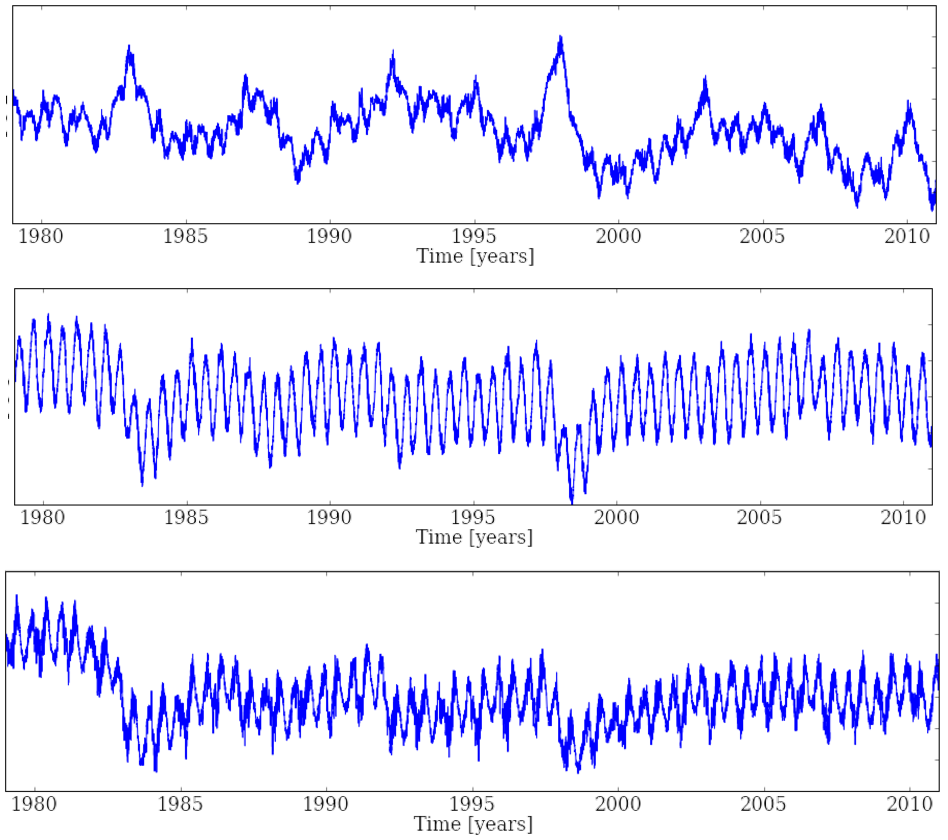
\includegraphics[width=.9\columnwidth]{images/climate_timeseries.pdf}
    \caption{In order from top to bottom, the timeseries for modes 3, 6, and 7 of the CFSR ocean temperature field.}
        \label{fig:climate_timeseries}
  \end{figure} 

  \begin{figure}[h!bt]
    \centering
    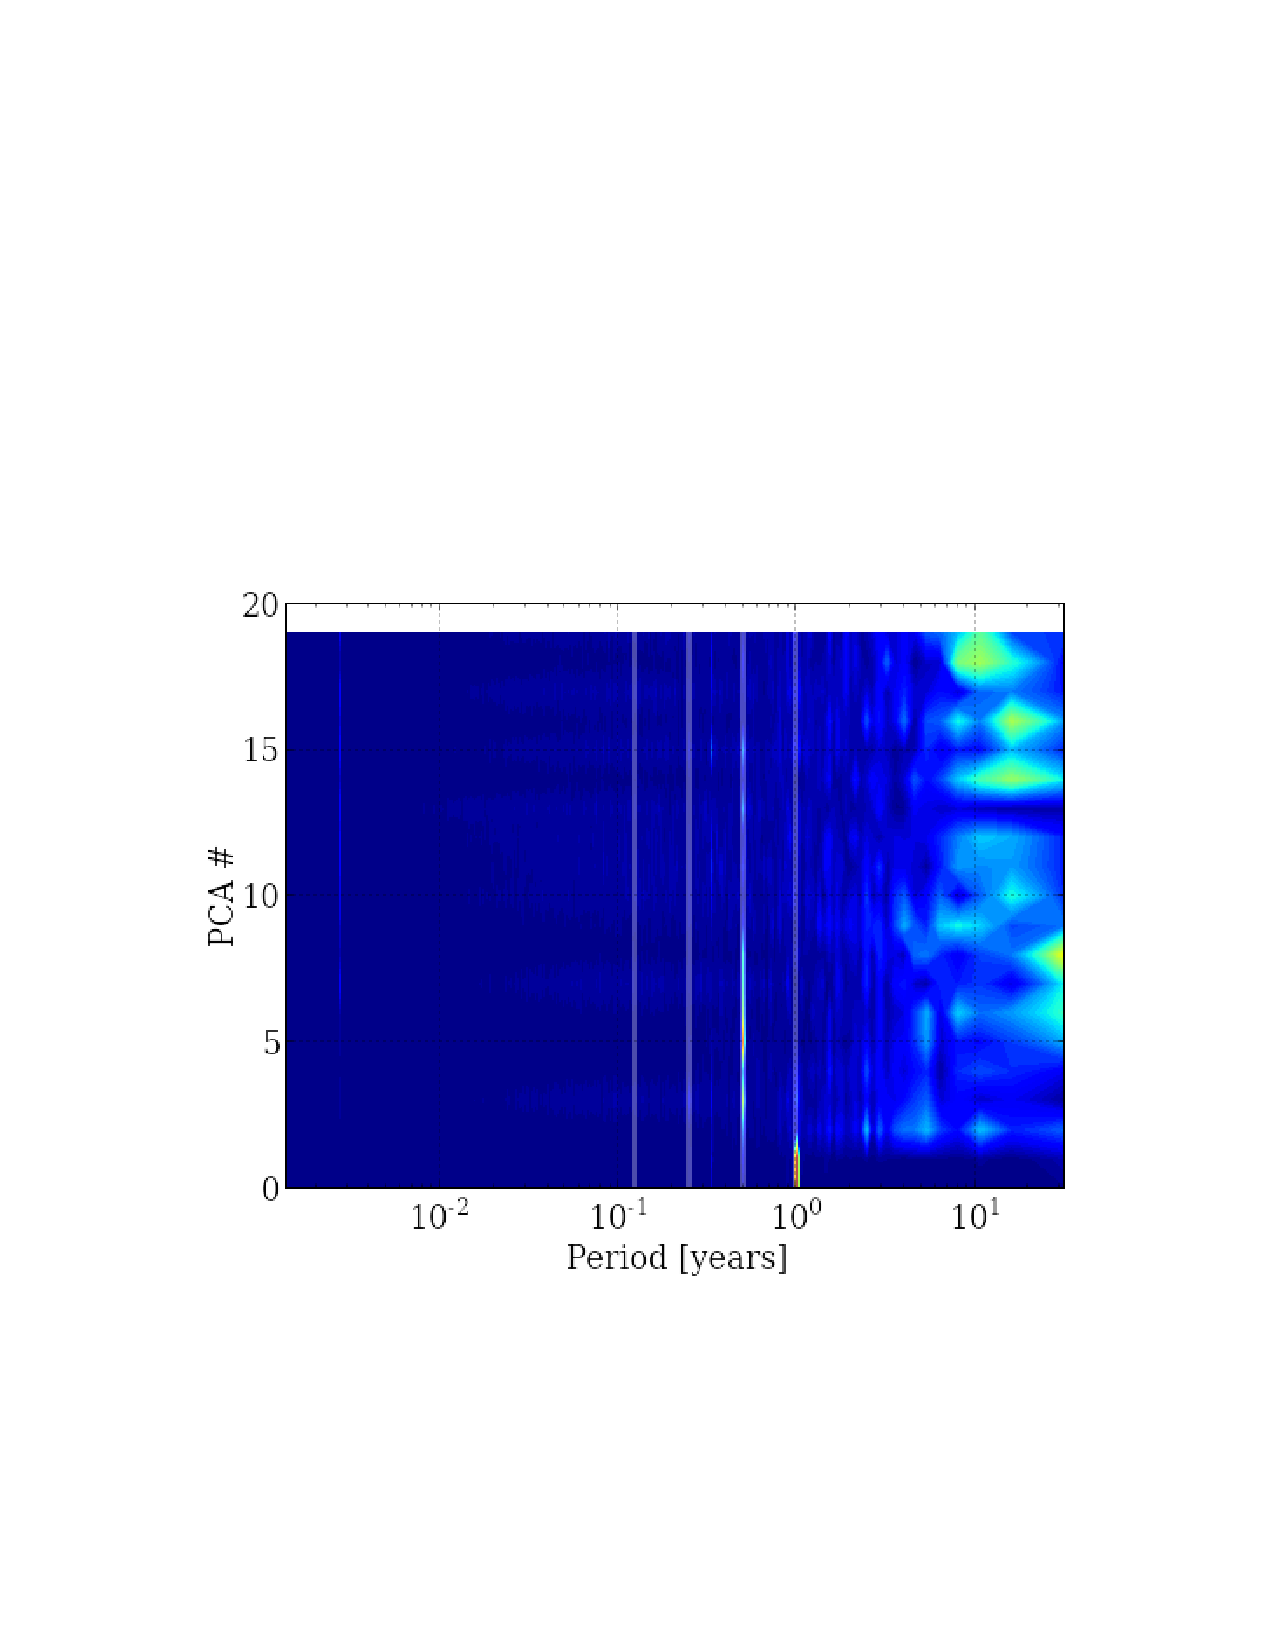
\includegraphics[width=.9\columnwidth]{images/climate_spectra.pdf}
    \caption{The power spectra of the first 20 modes of the CFSR ocean temperature field.}
    \label{fig:climate_spectra}
  \end{figure} 
The first two EOFs fully capture the annual cycles, so in
Figure~\ref{fig:climate_timeseries}, we present the time series corresponding to the
third, sixth, and seventh modes. The time series show the chaotic nature of the
large-scale modes of variability in the ocean, as well as the dominant
periodicities. Further, they show abrupt changes due to the 1983 ENSO,
and more significantly, the record-breaking ENSO of 1997--98.

The power spectra in Figure~\ref{fig:climate_spectra} show which modes contribute to
the low and high frequency modes of variability, and their relative dominance.
Note that, as mentioned above, the first two modes fully capture the annual
cycle, while the higher modes contain low frequency content. The intermediate
modes contain a complex interplay of various timescales, which is currently
under investigation.  

\begin{figure*}[h!bt]
  \centering
  \begin{subfigure}{.3\textwidth}
    \centering
    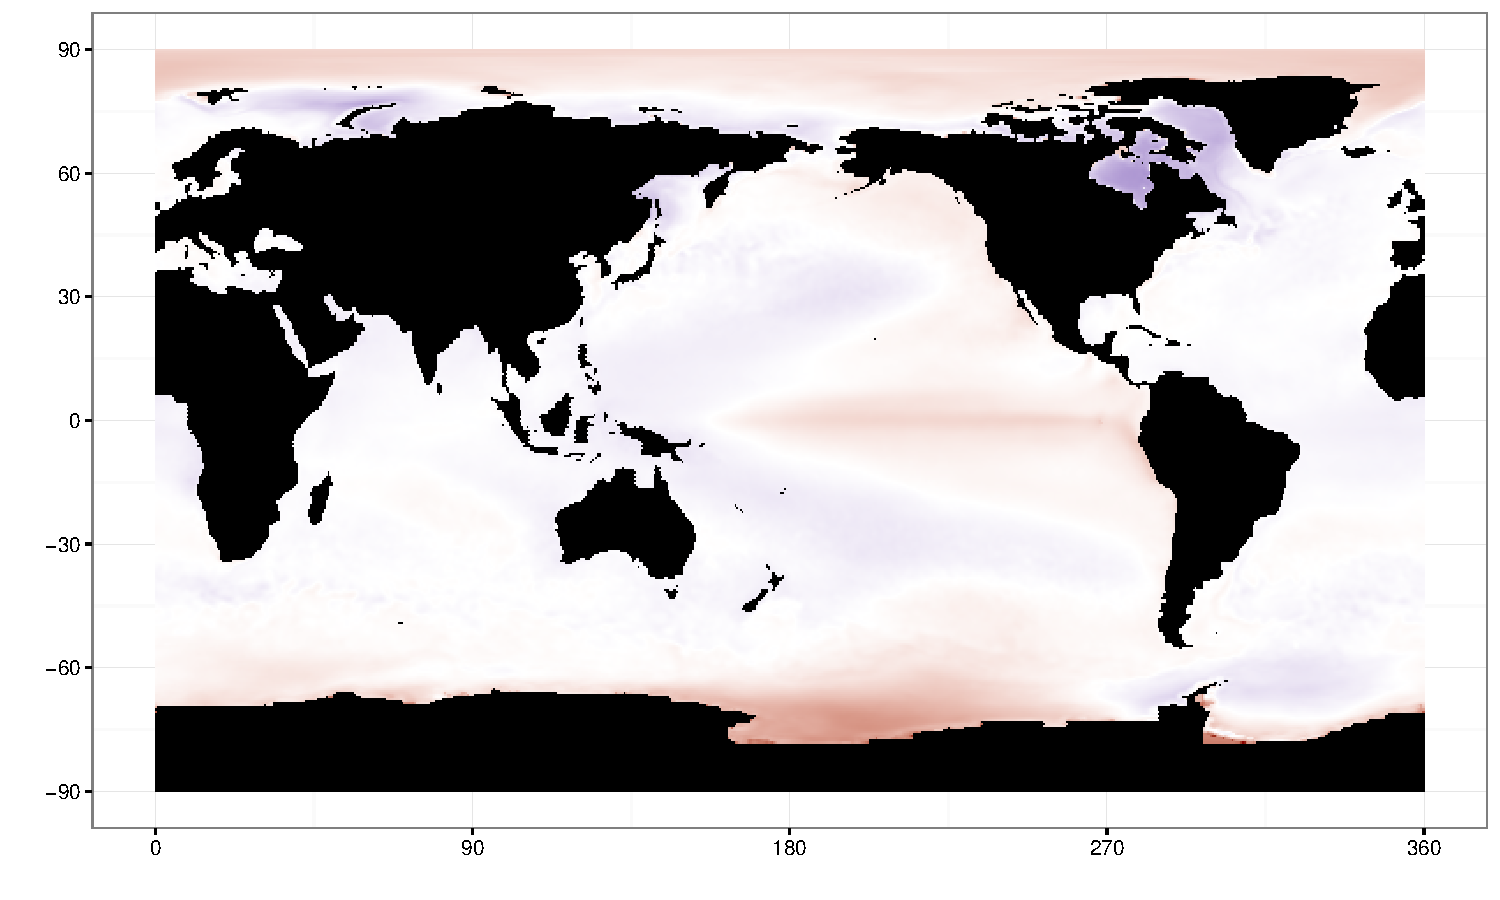
\includegraphics[width=.9\linewidth]{images/EOF3_0.pdf}
  \end{subfigure}
  \begin{subfigure}{.3\textwidth}
    \centering
    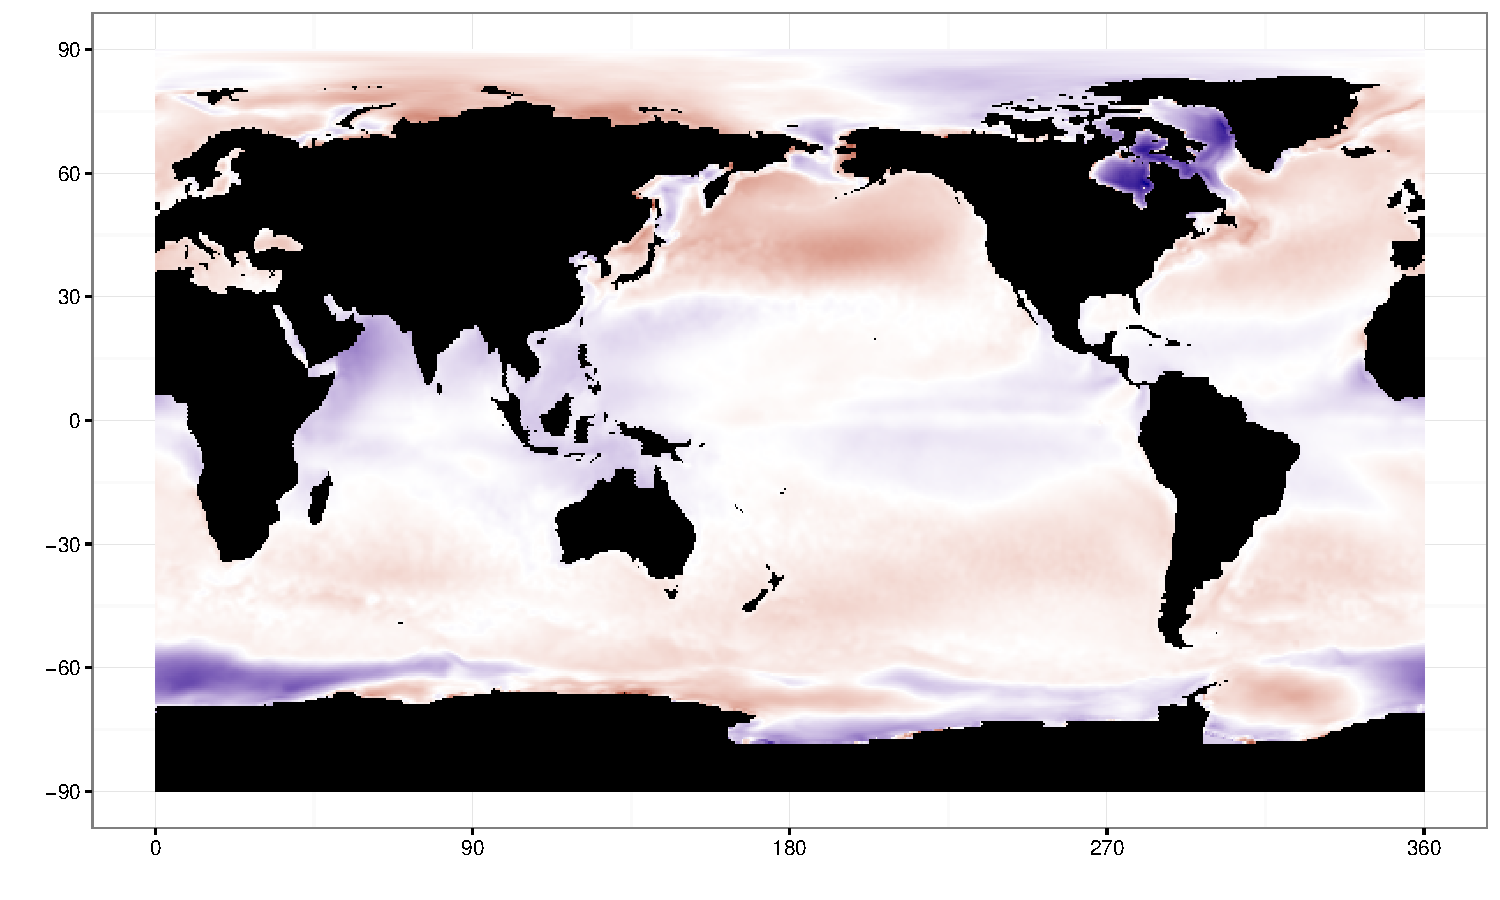
\includegraphics[width=.9\linewidth]{images/EOF6_0.pdf}
  \end{subfigure}
  \begin{subfigure}{.3\textwidth}
    \centering
    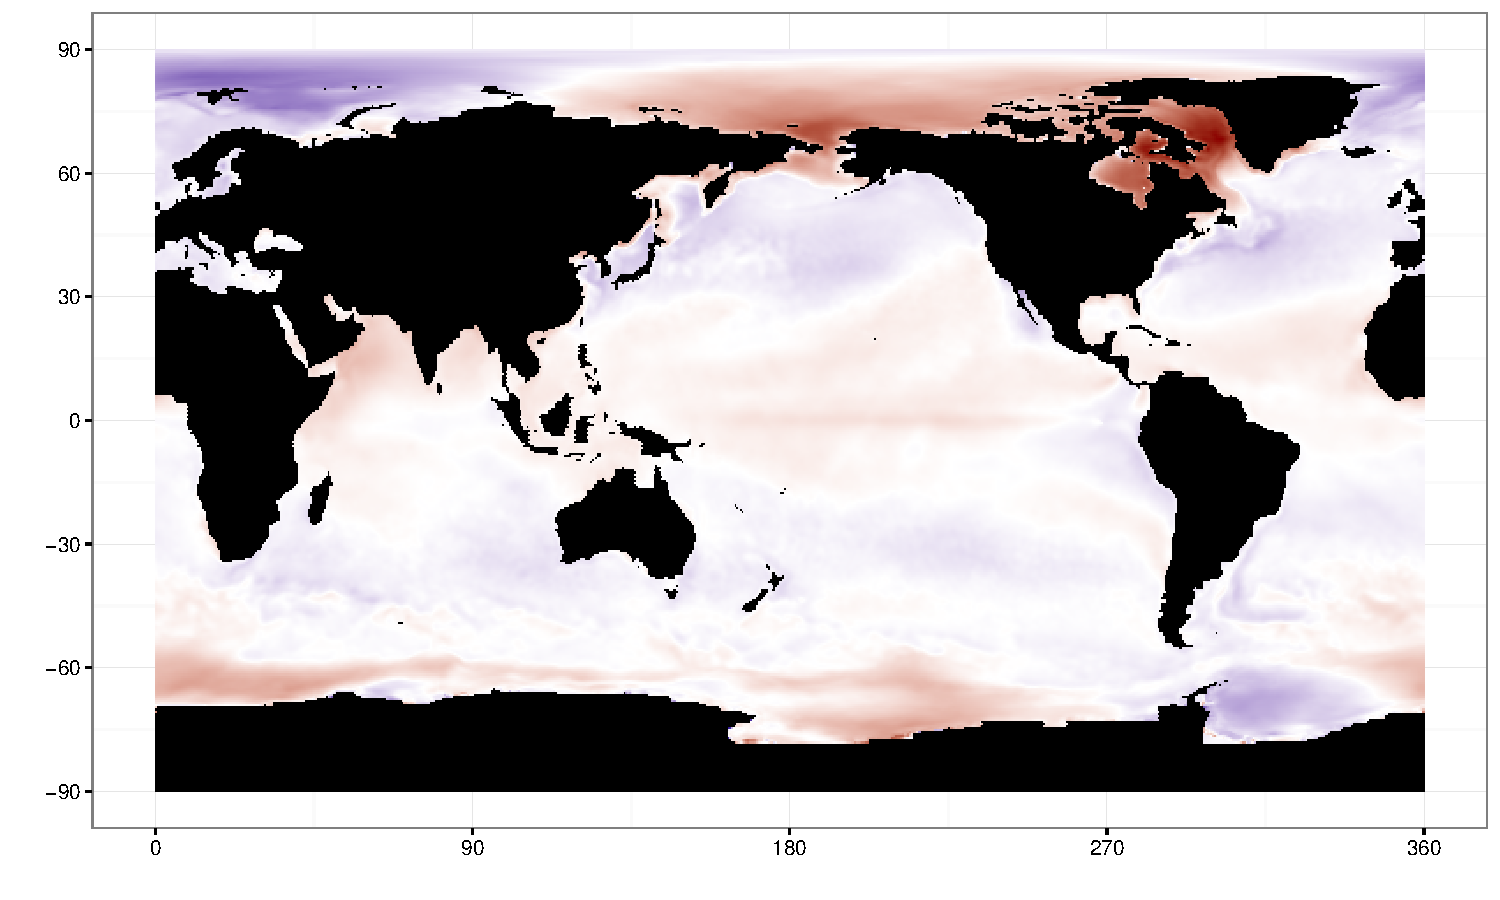
\includegraphics[width=.9\linewidth]{images/EOF7_0.pdf}
  \end{subfigure}
  \begin{subfigure}{.3\textwidth}
    \centering
    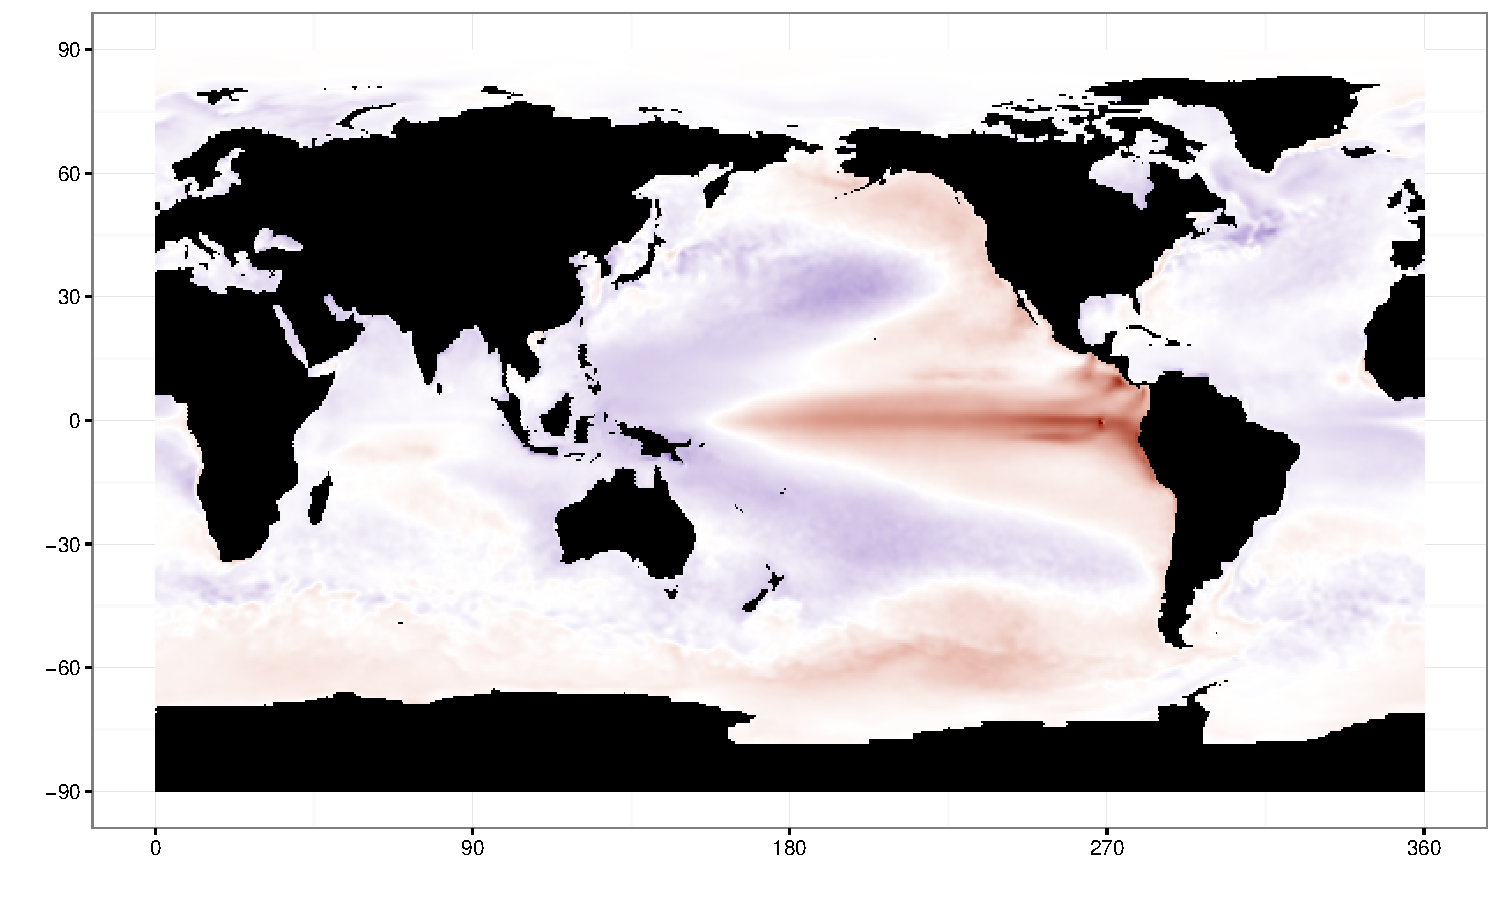
\includegraphics[width=.9\linewidth]{images/EOF3_55.pdf}
  \end{subfigure}
  \begin{subfigure}{.3\textwidth}
    \centering
    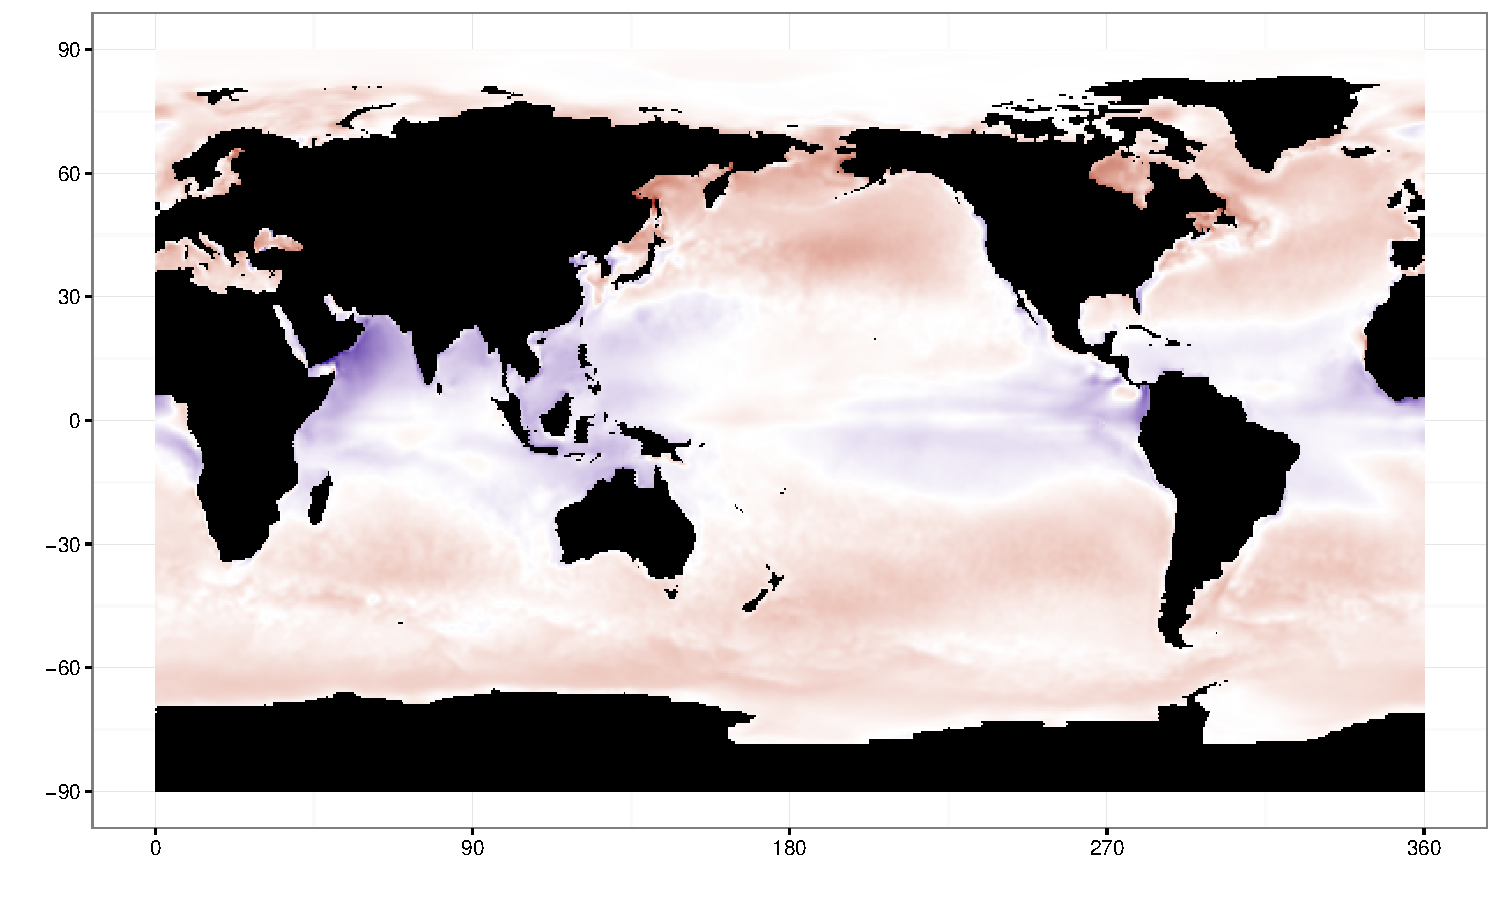
\includegraphics[width=.9\linewidth]{images/EOF6_55.pdf}
  \end{subfigure}
  \begin{subfigure}{.3\textwidth}
    \centering
    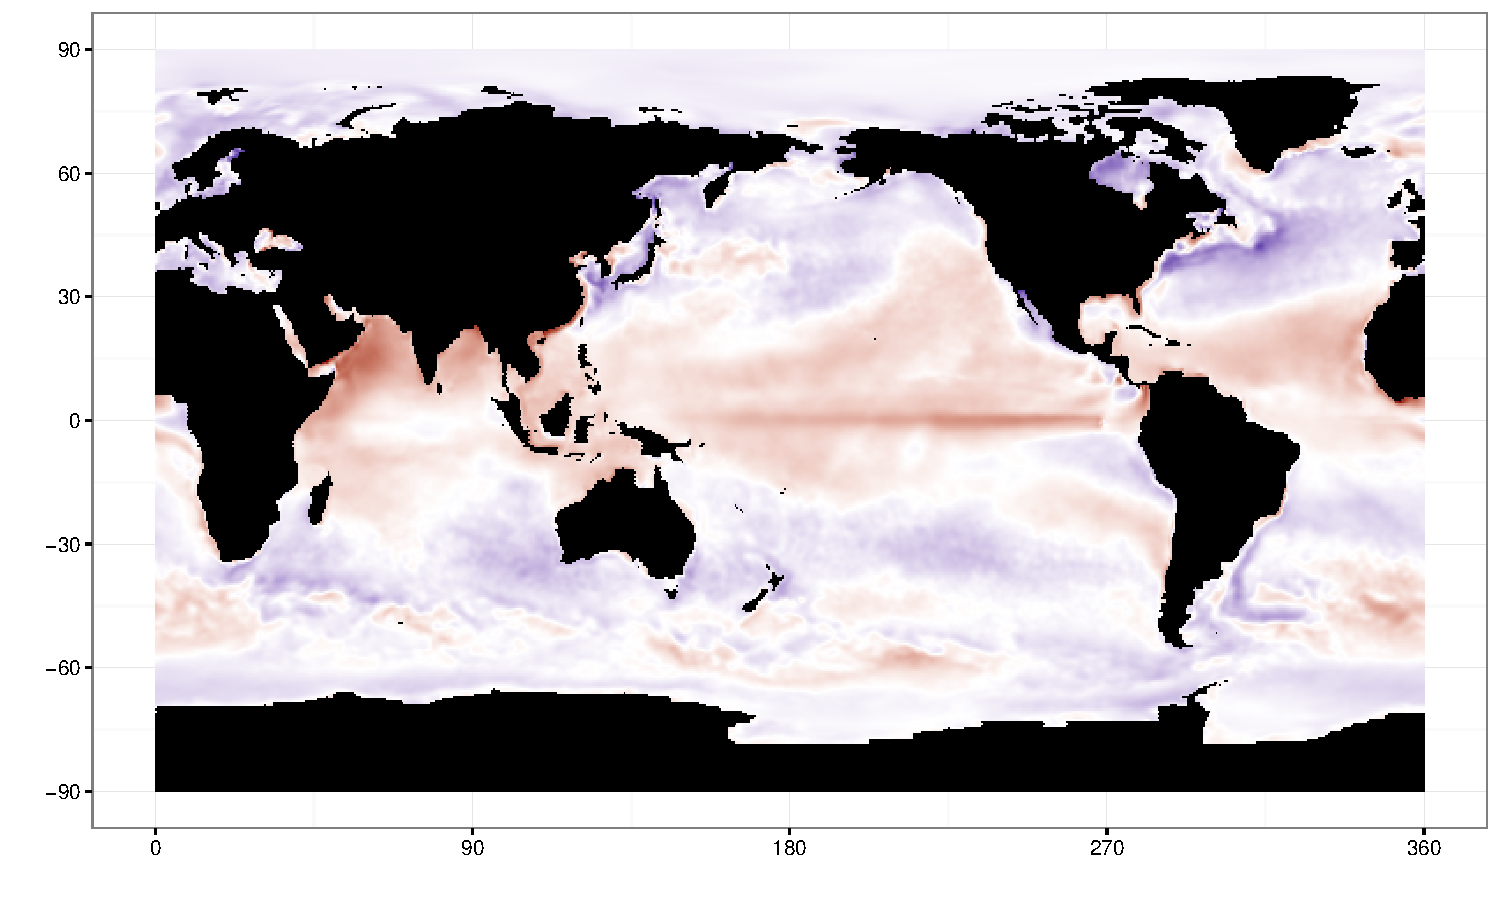
\includegraphics[width=.9\linewidth]{images/EOF7_55.pdf}
  \end{subfigure}
  \begin{subfigure}{.3\textwidth}
    \centering
    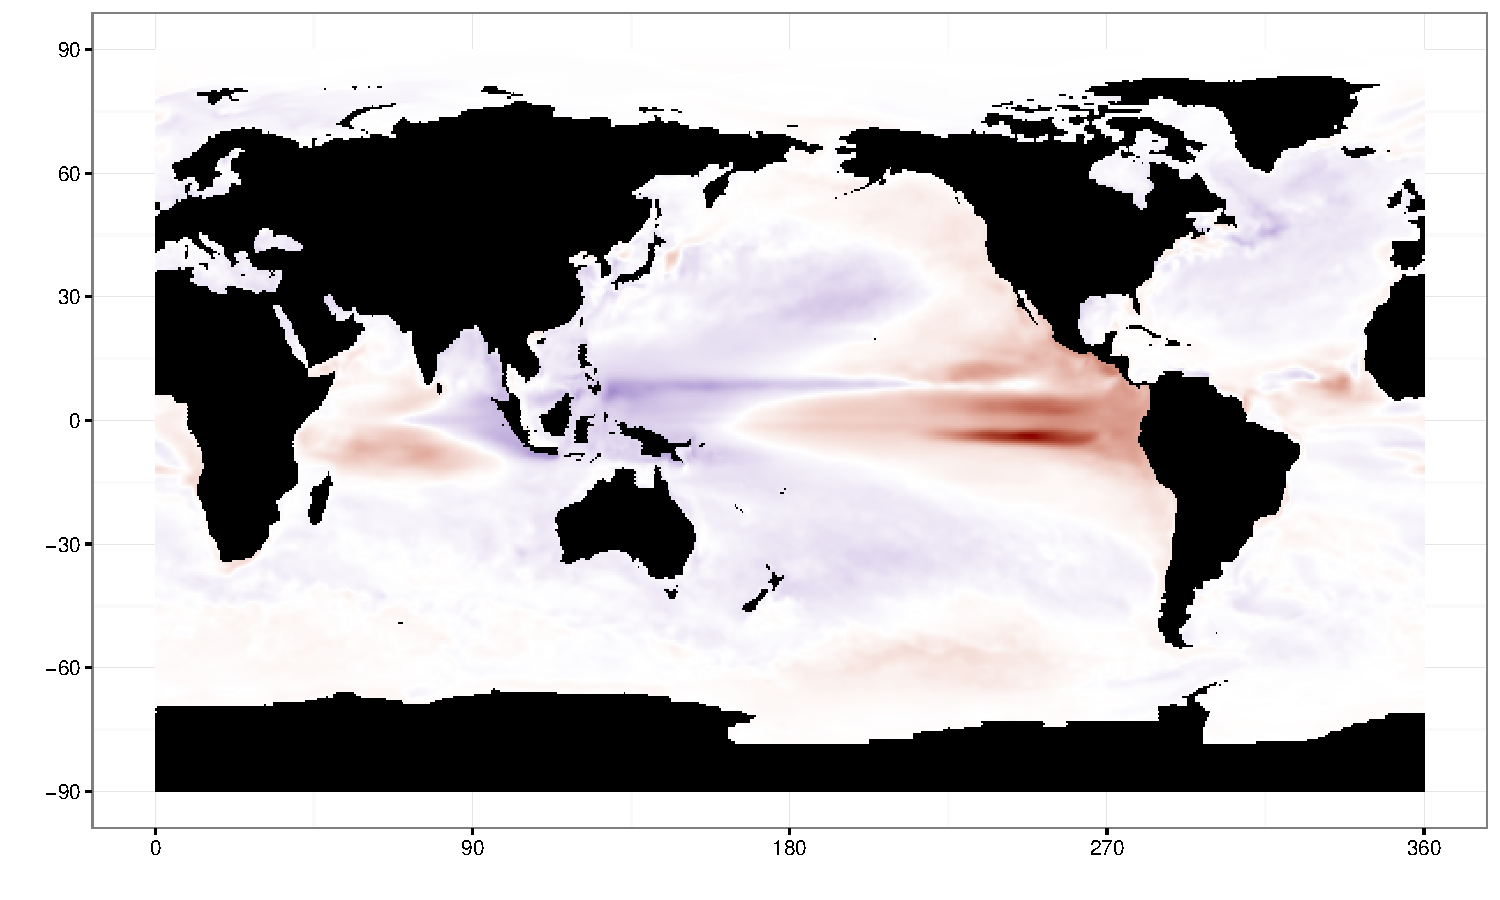
\includegraphics[width=.9\linewidth]{images/EOF3_135.pdf}
  \end{subfigure}
  \begin{subfigure}{.3\textwidth}
    \centering
    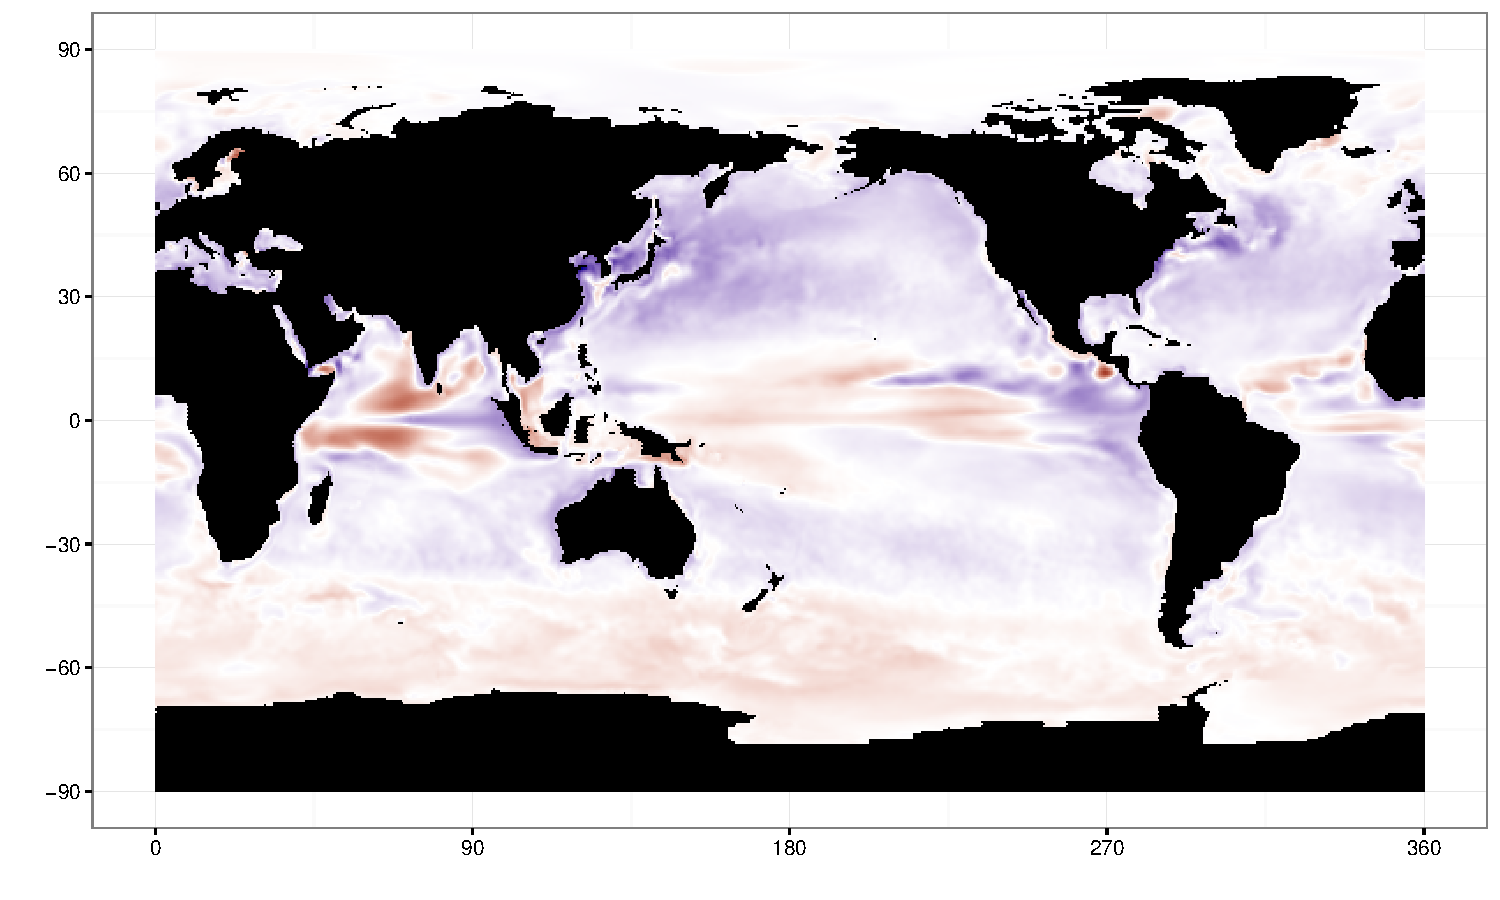
\includegraphics[width=.9\linewidth]{images/EOF6_135.pdf}
  \end{subfigure}
  \begin{subfigure}{.3\textwidth}
    \centering
    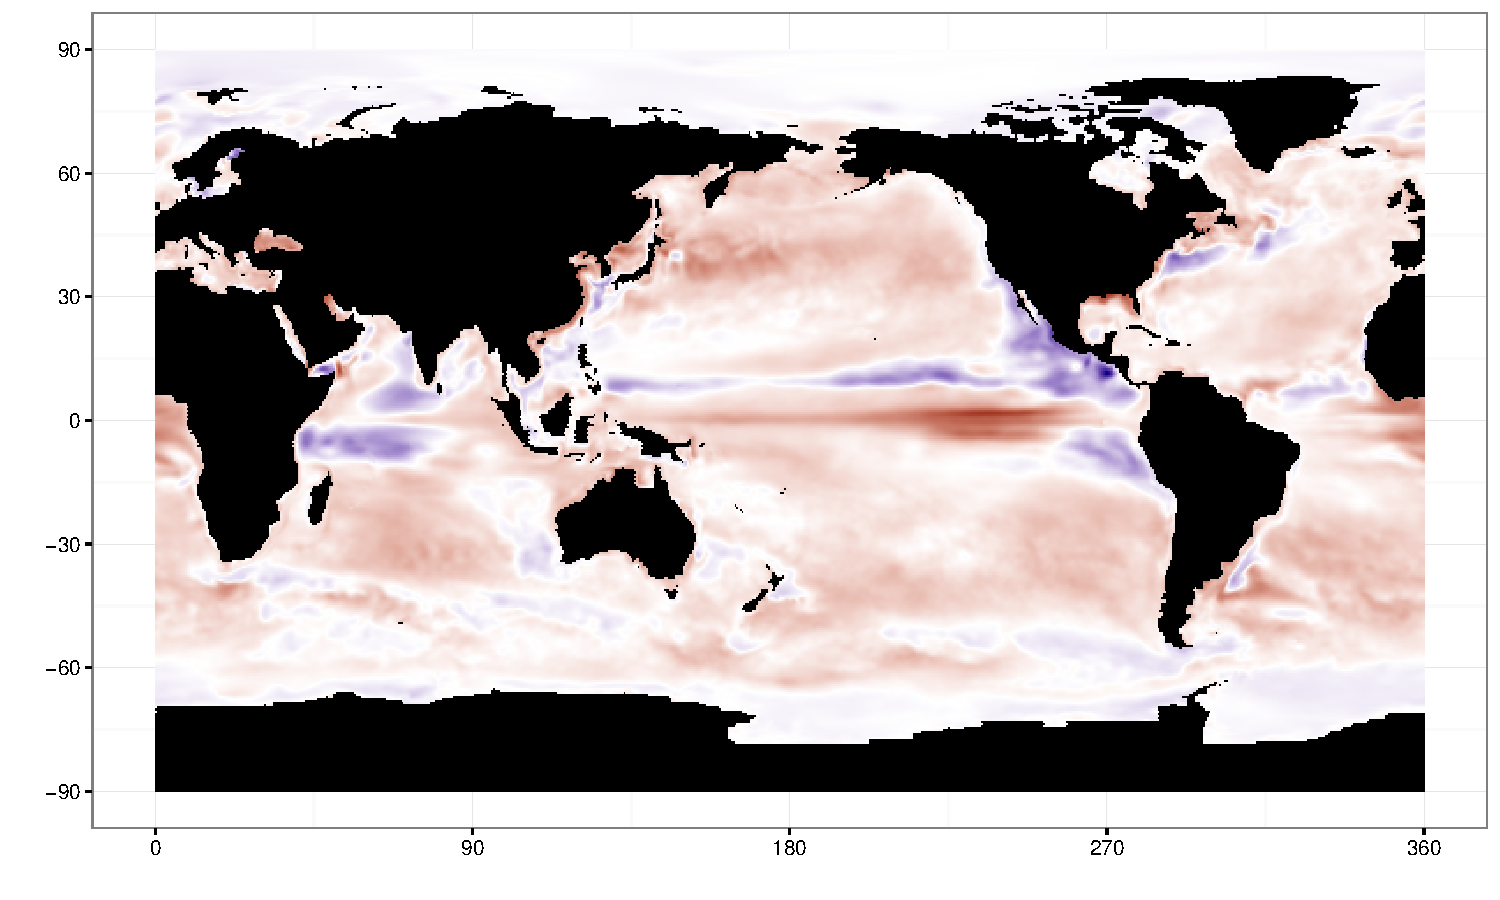
\includegraphics[width=.9\linewidth]{images/EOF7_135.pdf}
  \end{subfigure}
  \caption{Left to right, the mode 3, 6, and 7 spatial EOFs of the CFSR ocean temperature field at, from top to bottom, the surface, a depth of 55 meters, and a depth of 135 meters. }
  \label{fig:spatialEOFs}
\end{figure*}

The spatial EOF patterns in Figure~\ref{fig:spatialEOFs} show the relative
dominance of the Indian Ocean Dipole and the classic warm pool -- cold tongue
patterns of ENSO at various depths below the ocean surface. Note that the
dynamic near the thermocline is most dominant, rather than that closer to the
surface. Further, note that there are several smaller scale features that
have a strong influence at different depths. Work is on going to understand
the nature of these different spatial patterns and the factors that influence
their relative dominance.

  \subsection{Improving Spark on HPC Systems}

  \label{sect:lessons}
  
  The differences in performance between the Cray{\textsuperscript{\tiny\textregistered}}~XC40{\textsuperscript{\tiny\texttrademark}} system~\cite{alverson2012cray,craycascadesc12} and the experimental Cray cluster point to optimizations to Spark that could improve its performance on HPC-style architectures.  The two platforms have very similar configurations, with the primary difference being the lack of local persistent storage on the XC40 nodes.  As described in Section~\ref{sect:h2h}, this forces some of Spark's local scratch space to be allocated on the remote Lustre file system, rather than in local storage.  To mitigate this, and keep more of the scratch data local, we propose the following future work:
\begin{itemize}
  \item Spark cleans its local scratch space inefficiently.
  In particular, shuffle data is not immediately cleaned up after a shuffle
  completes. This makes fault recovery more efficient, but results in higher
  storage requirements for scratch space. A more efficient cleaning process would
  make it more feasible to fit the scratch data entirely in a local RAM disk and
  avoid using Lustre.
\item Spark does not currently allow you to configure primary and backup
  scratch directories.  Instead you list all scratch directories in a single
  list, and it distributes data in a round robin fashion between them as long
  as space is available.  You can bias it towards one storage device (e.g., RAM
  disk vs. Lustre) by listing multiple directories on the preferred device.
  Ideally, though, we would like to use a RAM disk (or other local storage)
  exclusively unless and until it fills, and only switch to Lustre directories
  if necessary.
\item Spark does not allow you to specify that a scratch directory is globally
  accessible.  Thus non-cached data is stored to the remote Lustre directory by
  the sender, and then later retrieved by the sender and sent to the receiver.
  This wastes a step, since the receiver could easily fetch the data directly
  from Lustre (or any other global file system).
\item Alternatively, a push model of communication (as opposed to the current
  pull model) might be possible - however this would have implications for
  reliability and the handling of very large data sets.\footnote{Storing the
    shuffle data to a large persistent block storage device and only sending
    it as needed allows Spark to easily shuffle more data than could fit in
    the remote buffers.  In a push-based model, extra logic and synchronization
    would be necessary to ensure that the remote buffers do not overflow.}
\end{itemize}


